\section{Preliminaries} \label{sec:preliminary}

In this section, we will describe the background of ReRAM technology, switching mechanism of the device and characteristics of retention failure observed in some ReRAM resistance states.

\begin{figure}[t]
\centering
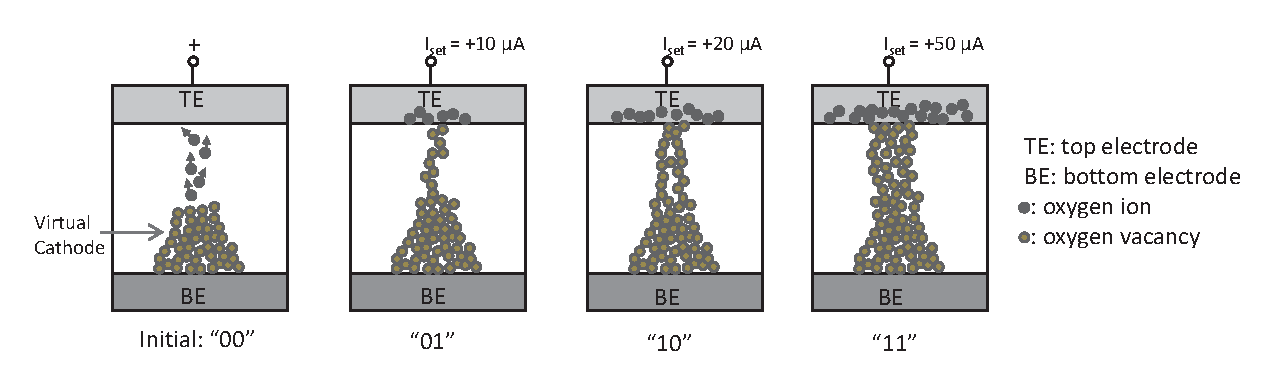
\includegraphics[width=0.48\textwidth]{fig/h2lview}
\vspace{-10pt}
\caption{Conceptual view of H2L programming.}
\label{fig:h2l}
\vspace{7pt}
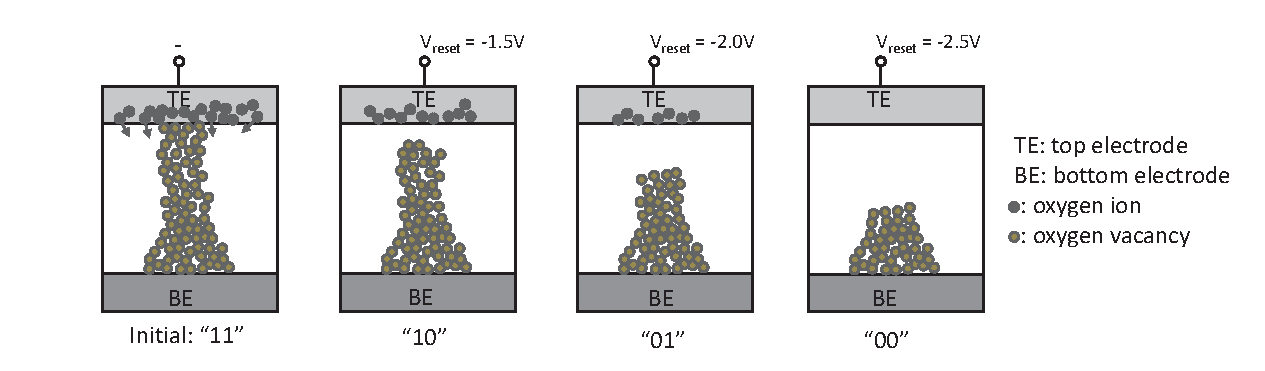
\includegraphics[width=0.48\textwidth]{fig/l2hview}
\vspace{-10pt}
\caption{Conceptual view of L2H programming.}
\label{fig:l2h}
\end{figure}

\subsection{Background of ReRAM technology}
The basic structure of a ReRAM cell is a metal layer sandwiched between two metal electrodes, called metal-insulator-metal (MIM) structure. The switching from HRS to LRS is defined as SET operation while the opposite process is RESET operation. The switching modes of ReRAM can be broadly classified into two modes: unipolar and bipolar. Unipolar means SET/RESET operation only depends the amplitude of the applied voltage/current but not on the polarity. Bipolar means SET and RESET occurs at different polarity. The switching mechanism and characteristics does not only depend on the choice of metal oxide layer but also the electrode materials and their interfacial properties. Some of promising oxide materials include $H_fO_x$, $T_iO_x$, $T_aO_x$, $N_iO_x$. An extremely fast switching ($<0.3ns$) has been reported for $H_fO_x$-based ReRAM [?ITRI?] and its endurance bar was recently raised to $10^{12}$ [??]. $T_aO_x$-based ReRAM has also demonstrated nanosecond switching [??] with endurance greater than $10^{12}$ [??]. $T_iO_x$ was interesting because of its intrinsic nonlinearity provides a low-cost solution for building crosspoint structure[?HP?]. Among all the ReRAM technologies, $H_fO_x$ seems to be have balanced metrics in switching time, switching energy, resistance ratio and endurance. Later in our case studies we will use $H_fO_x$-based ReRAM as an example. However, the discussion and solution we will have can be broadly applied for most ReRAM technologies with MLC capability.

\begin{figure}[t]
\centering
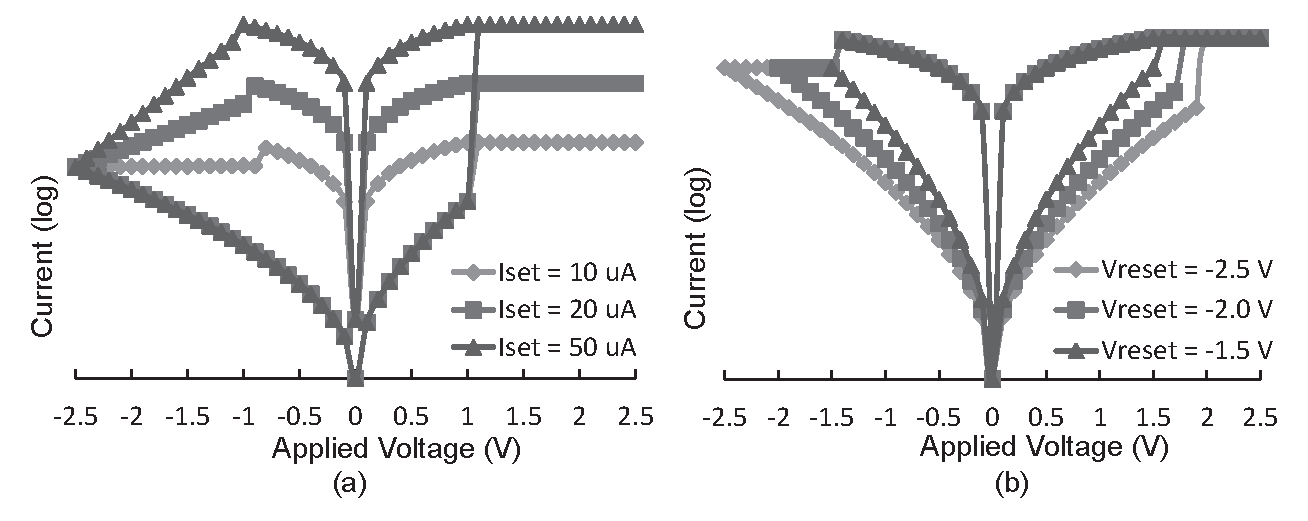
\includegraphics[width=0.48\textwidth]{fig/i-v}
\vspace{-10pt}
\caption{I-V curves demonstrate MLC characteristics of (a) H2L programming and (b) L2H programming.}
\label{fig:memristor}
\vspace{-15pt}
\end{figure}

The triggering of switching behavior of ReRAM is closely related to the formation or rupture of so-called conductive filament (CF), which consists of oxygen filaments. Once a filament is created inside the metal oxide layer and connects top electrode with bottom electrode, electrons can hop through the CF resulting in a LRS of the cell. The strength of the CFs is determined by the diameter or the number of CFs. The stronger (larger or more number of) the CFs are formed, the lower resistance the LRS is. Similarly, the rupture of CFs disconnects two metal electrodes and create a HRS of the cell. The resistance of the HRS is roughly proportional to the rupture length of CFs. Figure ? illustrates the formation process of the CFs in a ReRAM cell and the controlling of CF strength by adjusting the amplitude of SET current. When a positive current passing through the cell, the oxygen atoms are knocked out of the lattice and become negative-charged oxygen ion. The oxygen ions will be drift towards the anode and leaving corresponding oxygen vacancies in the metal oxide layer. CFs are formed when enough oxygen vacancies were created and connected as a conductive path. As we can see from the figure, stronger CFs are formed when more SET current pass though the cell for the same amount of time. This is the fundamental reason that a ReRAM cell can be programmed into intermediate levels of LRS, enabling the feasibility of MLC. The programming approach is defined as H2L (HRS-to-LRS) programming. The completely opposite MLC programming direction is to vary the RESET voltage so that the rupture length of the CFs can be controlled, as seen in Figure ?. When a RESET voltage is applied cross the ReRAM cell in LRS, oxygen ions migrate back to the metal oxide layer and combine with oxygen vacancies. For unipolar ReRAM, this is primary due to Joule heating. For bipolar ReRAM, the migration of oxygen ions is assisted by both thermal diffusion and a reverse dielectric field. As the RESET voltage is ramped up, the HRS resistance is increased due to increased rupture length of the CFs. This process is defined as L2H (LRS-to-HRS) programming.

Multi-step write-and-verify scheme is required in MLC ReRAM programming due to the existence of  both device-to-device variation and cycle-to-cycle variation. The device-to-device variation (or spatial variation) sources mostly from process variations (PVs) in device geometries and material properties. The impact of PVs on ReRAM was studied in [?DiminDAC?]. Stochastic switching behavior is the unique characteristic of ReRAM technology because the generation and degeneration of oxygen vacancies are naturally probabilistic and nondeterministic even under the same environment (i.e. electric field, oxygen concentration). That essentially means for a particular ReRAM cell, the resistance after the same SET current or RESET voltage has been applied for the same amount of time is difference from cycle to cycle. Using multiple pulses or a ramped series of pulses and introduce verification after each pulse helps improve the cycle-to-cycle uniformity [?123,124?]. The programming methodologies we propose later are all based on write-and-verify scheme for practical MLC applications.

\subsection{MLC read operation}

\subsection{Impact of Retention Failure on MLC reliability}
 Superior to SRAM and DRAM based on charge storage, emerging NVMs such as ReRAM and STTRAM are immune to soft errors caused by particle strike. However, each NVM technology still has non-zero "soft" (or recoverable) failure probability. The soft error of STTRAM can be caused by thermal fluctuations [?guangyuICCD?] and the failure rate increases as the thermal stability factor is lowered by PVs. The soft error of PCRAM relies on both short-term and long-term resistance drift [?free-p?], causing a well-known reliability issue of MLC PCRAM. Unlike the gradual resistance drift in PCRAM, a sudden resistance transition may occur in a ReRAM cell[?Bin?]. The sudden transition from HRS to LRS is referred as a HRS retention failure while the opposite transition is referred as a LRS retention. The retention failure essentially share the same principle with normal switching behavior or ReRAM - formation and rupture of CFs. For example, HRS failure is due to the generation of oxygen vacancies by a thermal activation process, which is a random process and requires much more time than typical write operation. [?Bin?] concludes that for ReRAM with large SET current ($>500\mu A$), strong CFs are formed (SET) or ruptured (RESET). In that case only HRS retention failure is observed because ruptured CFs are more like to be reconstructed. In contrast, for ReRAM with small SET current ($<100\mu A$) [?Shimeng?], only LRS retention failure is observed because weak-formed CFs are more likely to be ruptured due to the random degeneration of oxygen vacancies in the CFs. The test results in [?JubongPark?] in confirms that there exists reverse linear dependence between LRS resistance and retention failure time: $t_{failure }\propto 1/R_{LRS}$. Therefore, we identify, for the first time, the reliability issue in MLC ReRAM applications: in H2L programming higher LRS resistance levels are associated with weak CFs and are vulnerable to LRS retention failure; in L2H programming most HRS resistance levels are with strong CFs and are vulnerable to HRS retention failure.
